    \subsection{Análise de Processos}\label{sub:processos}

        Uma das tarefas delegadas ao presente estagiário foi também a análise de processos de OS. Dentro do Service center é possível analisar nas abas ``Monitoring'' e ``Processes'' os processos da aplicação e como é que estes foram concluídos ou em que estado estão, na Figura \ref{fig:interface_processo_servicecenter} pode-se ver a interface da plataforma ao visualizar os detalhes de um processo.

        Os processos aqui analisados são processos que acabavam suspensos, muitas vezes bastante antigos. São processos que causariam problemas a utilizadores se estes interagissem com o contrato específico associado a este processo, frequentemente podiam ser recomeçados e continuariam normalmente, mas em muitas das situações isto não acontece, esta situação oferece a possibilidade de identificar problemas com a plataforma e possíveis erros a resolver.

        \begin{figure}[H]
            \centering
            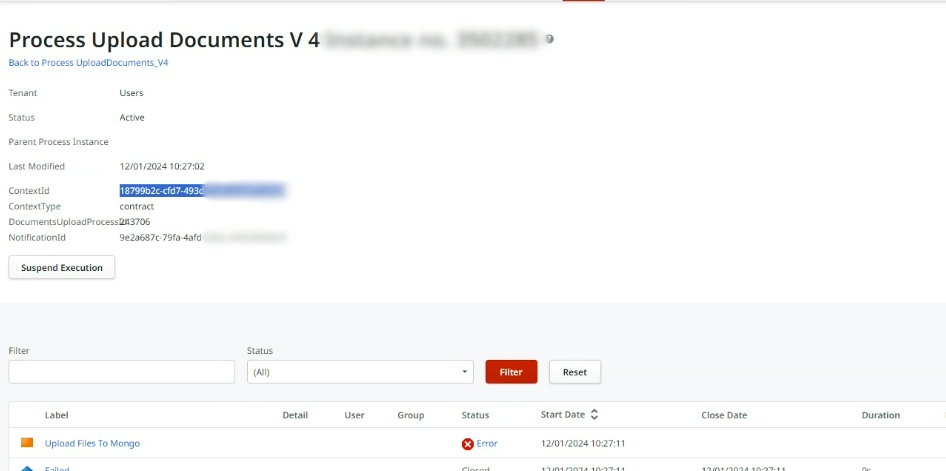
\includegraphics[width=\textwidth]{imgs/ProcessoServiceCenter.png}
            \caption{Interface de análise de um processo - Service Center}\label{fig:interface_processo_servicecenter}
            \source{Service Center Interno}
        \end{figure}

        Todos os processos revistos, independentemente do seu estado, tinham que ser anotados num documento de Excel específico para a tarefa com informação dos IDs dos contratos, \textit{placements}, equipas e utilizadores associados ao processo, bem como os erros ocorridos, caso tal seja relevante.

        Devido à natureza frequentemente repetitiva da análise destes, foi elaborado um web scraper em python que auxiliou na análise de alguns processos, por exemplo, foi automatizado o caso em que o processo \texttt{GenerateMRCEmailProcess} estava associado a um utilizador que estivesse inativo, registando e clicando ``skip'' na plataforma automaticamente, para mais informações refira à Secção \ref{secsec:scriptspython}.

        Existem três tipos de processos que geravam erros e era preciso analisar:

        \subsubsection{\texttt{SDC\_Generation}}\label{secsec:sdc_generation}

            % Isto é por causa da equipa de SDC para não sobrecarregarem

            Possivelmente o mais difícil de se analisar dos processos aqui representados.

            Foi imposto um limite de dez processos por hora e cinquenta por dia dos recomeçados com sucesso, de forma a não sobrecarregar a equipa dos processos.

            OS erros levantados neles tinham origem nos stamps das negociações e das suas complexidades. Devido à sua natureza volátil, e a criarem \textit{roles} diferentes para utilizadores e terem uma lógica de pertença a utilizadores e organizações pouco intuitiva, a sua ocorrência dependia de várias contingências.

            Em cada processo analisado era necessário encontrar a negociação e os stamps associados e fazer uma análise do campo \texttt{sdc\_enable} de cada stamp. Caso houvesse pelo menos um com a valor lógico verdadeiro para este campo, tentava-se correr de novo o processo, caso contrário, registava-se e não se tentava correr.
            
            Os processos podiam acabar numa das seguintes formas:
            \begin{itemize}
                \item \textbf{Closed}: Quando o processo correu de novo e concluiu com sucesso;
                \item \textbf{Error}: Quando acontecia um erro na execução, o erro era extraído e registado atempadamente;
                \item \textbf{Active --- Loop}: Quando fica num estado cíclico, por vezes durante horas. Na maior parte destes casos os processos acabariam por ficar suspensos de novo.
            \end{itemize}

        \subsubsection{\texttt{GenerateMRCEmailProcess}}\label{secsec:generate_mrc_email_process}

            Os processos \texttt{GenerateMRCEmailProcess} envolvidos na geração dos documentos MRC (\textit{Mutual Responsibility Contract}). O erro mais recorrente neste processo era identificado pela mensagem ``There was a technical issue sending the notification to the user <ID>''. Após uma análise detalhada do fluxo de ações nos logs do Azure, identificou-se que este problema ocorre quando uma ação tenta aceder a um documento na base de dados que não tem o campo URI preenchido, indicando a falta da referência ao documento na plataforma Nuxeo. A solução recomendada, caso um utilizador se depare e reporte o problema, é solicitar ao utilizador que execute a ação ``cancel and replace''.

            Outro erro detetado seria o identificado pela mensagem ``Invalid Username and password''. Neste caso, era feita uma validação para verificar se o utilizador estava inativo na base de dados. Se estivesse, era pressionado o botão ``skip'' no processo, pois não havia ações adicionais a serem tomadas. Caso o utilizador estivesse ativo, a informação era anotada e o estado atual era mantido. Eventualmente, poder-se-ia verificar nos logs do Azure as ações executadas até ocorrer o erro para identificar a ação que o causou.

            % Erro mais comum: There was a technical issue sending the notification to the user <ID>
            % Depois de revisto o fluxo de ações chamadas nos logs do azure, foi possível perceber que o erro ocorre quando uma ação chama um documento que na base de dados não tem o uri preenchido, ou seja não tem referenncia ao documneto.
            %A solução se um user se queixar seria pedir são utilizador para fazer cancel and replace.

            % Tinham outro erro: Invalid Username and password, e aqui é que faziamos a validação de se o user está inativo ou não: ver na Base de dados o utilizador, Se estiverem Inativos, ent davamos skip, não há nada a fazer, dar skip, Caso se encontre um ativo anota-se e deixa-se como está (ou eventualmente ver no azure os logs das ações percorridas até dar o erro).

        \subsubsection{\texttt{UploadDocuments\_V4}}\label{secsec:uploaddocuments_v4}

            O processo \texttt{UploadDocuments\_V4} desempenha um papel na gestão de documentos da plataforma, é na sequência de uma asserção da integridade destes documentos na plataforma, que surgiu a necessidade de fazer a análise destes processos. 
            
            O principal objetivo é validar se um documento está presente no Nuxeo e na base de dados do OutSystems em sincronia, utilizando o identificador do documento.

            O procedimento envolve a consulta à base de dados MongoDB para verificar se o campo URI do documento está preenchido, indicando a existência do documento no Nuxeo, e confirmando na plataforma. Se o documento estiver presente, prosseguia-se com o botão ``skip''. Caso contrário, se não existir informação na base de dados MongoDB, a situação seria registada. Nos casos em que o contrato associado ao documento também não é encontrado, a ação ``skip'' seria considerada. É relevante notar que durante a duração relevante, não foi registado nenhum cenário onde o contrato existia num \textit{placement} mesmo sem ter um URI.

            % O objetivo seria ver se o documento está presente no Nuxeo e em OutSystems
            % Viamos na base de dados o documento atravez do ID
            % Queremos ver se o campo uri está preenchido com qualquer coisa, que se tiver quer dizer que existe no Nuxeo. Mas para confirmar podiamos ir mesmo ao Nuxeo: Copiavas o Uri e punhas no nuxio e deve aparecer
            % Se aparecer, podes clicar no skip:
            % Se não aparecer nada na base de dados MongoDB, Anotavam no Excel e não lhe mexíamos. Mas antes disso, procuravas o contrato, se o contrato não existisse também, aí podiam dar skip: 
            % O caso em que o contrato existe nunca foi encontrado antes!

                \subsubsection{Scripts de Automação em Python}\label{secsec:scriptspython}

            Com o intuito de otimizar a análise dos processos e mediante as adequadas autorizações concedidas, o estagiário assumiu a responsabilidade de automatizar a análise destes. Foram consideradas diferentes opções de interação com os APIs internos do Azure, OutSystems e MongoDB. Contudo, para obter acesso programático à base de dados de produção, seria necessário solicitar aprovação diretamente ao cliente, à RIL. Além disso, os APIs feitos para o Azure de produção não tinham um histórico favorável de funcionamento em Python, existiam apenas programados em C\#.

            Diante a situação, optou-se por se automatizar através da implementação de um web scraper e da interação direta com o navegador. Os scripts criados estão disponíveis no Anexo \ref{sec:scripts}.

            \subsubsubsection{User Stories}\label{secsecsec:us_python}

                Realizou-se assim um estudo das User Stories (US) a implementar, com o objetivo de reduzir ao mínimo os requisitos, garantir uma implementação rápida e alcançar um elevado nível de automatização. Este processo conduziu à identificação das US das tabelas \ref{table:python_us1}, \ref{table:python_us2}, \ref{table:python_us3} e \ref{table:python_us4}.

                \begin{table}[htbp] % htbp
                    \centering
                    \begin{tabularx}{1\textwidth}{|>{\raggedright\arraybackslash}X|}
                        \hline
                        \rowcolor{lightgray}
                        \textbf{User Story:} Análise de Processos SDC no Estado ``Active - Loop'' \\
                        \hline
                        \rowcolor{lightgray!20}
                                        
                        \begin{itemize}
                            \item \textbf{Visão:} Efetuar uma análise detalhada dos dados dos processos SDC presentes num ficheiro Excel local, identificando aqueles que se encontram no estado "Active - Loop". Posteriormente, realizar uma avaliação dos dados do processo e dos erros associados. A tarefa inclui a atualização do estado para "Suspended" no Excel, juntamente com o registo do tipo de erro e a URL correspondente.

                            \item \textbf{Como...} Utilizador autorizado a executar operações sobre os processos SDC no estado "Active - Loop".

                            \item \textbf{Eu quero...} Analisar os dados dos processos SDC no estado "Active - Loop", corrigir os erros associados, atualizar o estado para "Suspended" no Excel e registar informações detalhadas sobre o tipo de erro e a URL no mesmo ficheiro.

                            \item \textbf{Para quê...} Garantir uma gestão eficaz dos processos SDC, corrigindo problemas associados e mantendo um registo claro das ações realizadas para futura referência e auditoria.
                        \end{itemize}
                        \\
                        \hline
                    \end{tabularx}
                    \caption{Detalhes da US \textit{Análise de Processos SDC no Estado ``Active - Loop''}}\label{table:python_us1}
                \end{table}

                \begin{table}[htbp] % htbp
                    \centering
                    \begin{tabularx}{1\textwidth}{|>{\raggedright\arraybackslash}X|}
                        \hline
                        \rowcolor{lightgray}
                        \textbf{User Story:} Análise de Processos GenerateMRCEmailProcess com Utilizadores Inativos \\
                        \hline
                        \rowcolor{lightgray!20}
                                        
                        \begin{itemize}
                            \item \textbf{Visão:} Efetuar uma análise dos dados dos processos \texttt{GenerateMRCEmailProcess}, contidos num ficheiro Excel local, focando-se nos processos que possuem apenas o número na primeira coluna, sem informações adicionais. Utilizando a plataforma Atlas, identificar os processos que apresentam o utilizador inativo e, automaticamente, pressionar o botão ``skip'' na plataforma Service Center para cada um deles. Preencher sempre com os dados do processo no Excel.

                            \item \textbf{Como...} Utilizador autorizado a realizar operações relacionadas com os processos \texttt{GenerateMRCEmailProcess} e a aceder à plataforma Atlas.

                            \item \textbf{Eu quero...} Analisar os dados dos processos \texttt{GenerateMRCEmailProcess} presentes no ficheiro Excel, identificar os processos com utilizadores inativos através do Atlas e automatizar a exclusão destes processos na plataforma Service Center.

                            \item \textbf{Para quê...} Assegurar uma gestão eficiente dos processos \texttt{GenerateMRCEmailProcess}, evitando a interação com utilizadores inativos e otimizando o fluxo de trabalho no Service Center.
                        \end{itemize}
                        \\
                        \hline
                    \end{tabularx}
                    \caption{Detalhes da US \textit{Análise de Processos GenerateMRCEmailProcess com Utilizadores Inativos}}\label{table:python_us2}
                \end{table}
                
                \begin{table}[htbp] % htbp
                    \centering
                    \begin{tabularx}{1\textwidth}{|>{\raggedright\arraybackslash}X|}
                        \hline
                        \rowcolor{lightgray}
                        \textbf{User Story:} Análise de Processos \texttt{UploadDocuments\_V4} no Excel \\
                        \hline
                        \rowcolor{lightgray!20}
                                        
                        \begin{itemize}
                            \item \textbf{Visão:} Efetuar uma análise dos dados dos processos \texttt{UploadDocuments\_V4} presentes num ficheiro Excel local. Verificar se o ``ContextI'' dos processos não tem nenhum documento associado na base de dados de Produção do MongoDB. Em caso negativo, assinalar no Excel com a mensagem ``Contract does not exist in Mongo'' e prosseguir. Se existir, verificar se todos os documentos possuem um URI e, em caso afirmativo, assinalar no Excel com o comentário ``Document in Mongo''. A informação será sempre registada no Excel.

                            \item \textbf{Como...} Utilizador habilitado a executar operações relacionadas com os processos \texttt{UploadDocuments\_V4} e a aceder à base de dados de Produção do MongoDB.

                            \item \textbf{Eu quero...} Analisar os dados dos processos \texttt{UploadDocuments\_V4} no ficheiro Excel, verificar a existência de documentos associados ao ``ContextId'' na BD do MongoDB e assinalar no Excel as mensagens adequadas conforme as condições verificadas.

                            \item \textbf{Para quê...} Assegurar uma gestão precisa dos processos \texttt{UploadDocuments\_V4}, identificando casos em que o contrato não existe na base de dados do MongoDB ou verificando se todos os documentos possuem um URI, proporcionando um registo claro e informado no Excel.
                        \end{itemize}
                        \\
                        \hline
                    \end{tabularx}
                    \caption{Detalhes da US \textit{Análise de Processos GenerateMRCEmailProcess com Utilizadores Inativos}}\label{table:python_us3}
                \end{table}

                \begin{table}[htbp] % htbp
                    \centering
                    \begin{tabularx}{1\textwidth}{|>{\raggedright\arraybackslash}X|}
                        \hline
                        \rowcolor{lightgray}
                        \textbf{User Story:} Interrupção Controlada da Execução do Script \\
                        \hline
                        \rowcolor{lightgray!20}
                                        
                        \begin{itemize}
                            \item \textbf{Visão:} Permitir a interrupção controlada da execução do script a qualquer momento através da combinação de teclas CTRL + ALT + S.

                            \item \textbf{Como...} Utilizador precisa de interromper a execução do script de forma controlada e imediata.

                            \item \textbf{Eu quero...} Ter a capacidade de interromper o script em execução em qualquer ponto utilizando a combinação de teclas \texttt{CTRL} + \texttt{ALT} + \texttt{S}.

                            \item \textbf{Para quê...} Proporcionar ao utilizador um meio eficiente de parar a execução do script quando necessário, garantindo uma interrupção rápida e controlada, sem comprometer a integridade dos dados ou funcionalidade do sistema.
                        \end{itemize}
                        \\
                        \hline
                    \end{tabularx}
                    \caption{Detalhes da US \textit{Análise de Processos GenerateMRCEmailProcess com Utilizadores Inativos}}\label{table:python_us4}
                \end{table}

            \subsubsubsection{Requisitos Funcionais}\label{secsecsec:req_func_python}

                A partir das USs, foram derivados os requisitos funcionais, apresentados na tabela \ref{tab:req_func_python}. Estes requisitos representam as descrições e comportamentos externos exigidos pelo software, delineando as funcionalidades que o sistema deve cumprir. Proporcionam uma visão de alto nível do sistema.
                
                \begin{table}[htbp] % htbp
                    \centering
                    \begin{tblr}{
                        % example for tblr: https://tex.stackexchange.com/questions/603349/tabularray-and-new-command-for-multicolumn-cells
                        % another example: https://tex.stackexchange.com/questions/605676/tabularray-how-to-control-the-vertical-alignment-of-the-cells-contents
                        hlines={lightgray}, vlines={lightgray},
                        width = \linewidth,% total width set to width available
                        %rows = {c,m}, % c aligns horizontally, m aligns vertically, aligns all rows
                        colspec={X[1,c,m] X[5,l,m]}, % the first number is the size
                    }
                    % \textbf{Tempo trabalhado}
                        \textbf{ \# } & \textbf{Nome} \\
                        REQ-01 & Análise de Processos SDC \\
                        REQ-02 & Análise de Utilizadores Inativos em GenerateMRCEmailProcess \\
                        REQ-03 & Análise de Documentos em UploadDocuments\_V4 \\
                        REQ-04 & Interrupção Controlada do Script \\
                        REQ-05 & Pintar Colunas com Erros de Roxo para Análise Manual \\
            
                    \end{tblr}
                    \caption{Requisitos funcionais dos scripts para análise de processos}
                    \label{tab:req_func_python}
                \end{table}

                Na tabela \ref{tab:req1_py} está representado, a título de exemplo, um requisito funcional, está acompanhado de um resumo detalhado e descrição. A lista completa dos requisitos encontra-se disponível no Anexo \ref{sec:Req_func_python_anexo}.

                \begin{table}[htbp] % htbp
                    \centering
                    \begin{tblr}{
                        % example for tblr: https://tex.stackexchange.com/questions/603349/tabularray-and-new-command-for-multicolumn-cells
                        % another example: https://tex.stackexchange.com/questions/605676/tabularray-how-to-control-the-vertical-alignment-of-the-cells-contents
                        hlines={lightgray}, vlines={lightgray},
                        width = \linewidth,% total width set to width available
                        %rows = {c,m}, % c/l/r aligns horizontally, m/t/b aligns vertically, aligns all rows
                        colspec={X[1,l,m] X[5,l,m]}, % the first number is the size % the second is c for center, l for left
                    }
                    % \textbf{Tempo trabalhado}
                        \textbf{ Nome } & \textbf{REQ-01 --- Análise de Processos SDC} \\
                        Resumo                  & Este requisito visa permitir a análise detalhada dos processos SDC num ficheiro Excel local, focando-se na identificação e correção dos processos no estado "Active - Loop". \\

                        Descrição               & O sistema deve possibilitar a identificação dos processos SDC no estado "Active - Loop" num ficheiro Excel local. Após a análise, o estado destes processos deve ser atualizado para "Suspended", e informações detalhadas sobre erros e URLs associadas devem ser registadas no Excel. \\

                        Requisitos Relacionados & -- \\
            
                    \end{tblr}
                    \caption{Requisito funcional \textit{Análise de Processos SDC}}
                    \label{tab:req1_py}
                \end{table}

                Devido à simplicidade deste projeto, requisitos não funcionais não foram apurados.
                
            \subsubsubsection{Implementação e Arquitetura}\label{secsecsec:implementacao_python}

                Seguidamente, procedeu-se à implementação de três scripts distintos para os três primeiros casos de uso. Desta forma, foi desenvolvido um script para analisar cada tipo de processo: um para a análise dos processos SDC já concluídos, outro para a análise dos processos MRC cujos utilizadores se encontravam inativos, e um terceiro para a análise global dos processos Documents\_V4. Para isto foram utilizadas diversas bibliotecas em Python, incluindo:

                \begin{itemize}
                    \item \texttt{json}: Utilizada para lidar com a manipulação de dados em formato JSON;

                    \item \texttt{pyautogui}: Esta biblioteca foi empregada para automatizar a interação com a interface gráfica do utilizador (GUI) quando tal não era facilmente fazível através do driver selenium;
                    
                    \item \texttt{pyperclip}: Desempenha um papel crucial na transferência de dados entre a interface do navegador, mais especificamente, a plataforma Atlas e o código, facilitando a cópia e colagem de dados;
                    
                    \item \texttt{selenium}: Utilizado para a automação da interação com navegadores web, o \texttt{selenium} permite o controlo programático de um navegador, possibilitando a navegação através de páginas web, preenchimento de formulários,  extração de dados, etc;
                    
                    \item \texttt{BeautifulSoup}: Essencial para a análise e extração e interpretação de dados a partir de documentos HTML;
                    
                    \item \texttt{time}: Importante para gerir pausas e esperas durante a execução do script, embora sempre indesejável, sendo um método que deteta a prontidão dos elementos da página melhor, foi usado como uma alternativa nas situações em que se considerou adequado ou em situações de erro;
                    
                    \item \texttt{openpyxl}: Desempenhando um papel crucial na manipulação de folhas de cálculo Excel, o \texttt{openpyxl} permitiu a escrita e leitura das informações nos ficheiros Excel utilizados pelos scripts.
                \end{itemize}

            \subsubsubsection{Testes e Validações}\label{secsecsec:testes_validacoes_python}

                Realizaram-se testes unitários em cada função para assegurar a sua integridade durante o desenvolvimento, garantindo que cada componente do sistema funciona corretamente e em conformidade com os requisitos estabelecidos, proporcionando uma base sólida para a fiabilidade do código, isto é um método natural e uma peça fundamental do desenvolvimento. Através dos testes unitários executados, eram frequentemente encontrados erros nas funções e casos que precisavam de ser prevenidos.
            
        % Devido à natureza frequentemente repetitiva da análise destes, foi elaborado um web scraper em python que auxiliou na análise de alguns processos, por exemplo, foi automado o caso em que o processo \texttt{GenerateMRCEmailProcess} estava associado a um utilizador que estivesse inativo, registando e clicando ``skip'' na plataforma automáticamente, para mais informações refira à Secção \ref{secsec:scriptspython}.        

        \subsubsection{Documentação Criada}\label{secsec:documentação}
            
            Ao término do estágio, surgiu a necessidade de desenvolver uma página no Confluence englobando toda a informação acumulada ao longo do processo de reprocessamento dos procedimentos de produção. Com o intuito de garantir acessibilidade universal na RIL, esta página foi redigida em inglês, assegurando compreensão por qualquer membro da equipa. Detalhando minuciosamente o processo de análise de cada procedimento, desde a ativação das permissões de acesso até à configuração do VPN de Azure, a documentação oferece uma visão abrangente e detalhada do percurso seguido. 
            
            Foi também realizada uma reunião no final do estágio entre o estagiário e vários membros das equipas que ficariam encarregues da análise dos processos, isto para transferir a informação de forma direta e célere. Esta iniciativa, juntamente com a documentação adicionada, visou consolidar o conhecimento adquirido, facilitando o trabalho de futuros analistas e contribuir para a partilha eficiente de informações na organização. Foi criada também uma secção com uma explicação do uso dos scripts criados, estes foram adicionados aos ficheiros relacionados com processos de produção.

        
        



